\title{Scalar conservation laws with boundary condition}
\markright{Scalar conservation laws with boundary condition}

\author{By~ K. T. Joseph}
\markboth{K. T Joseph}{Scalar conservation laws with boundary condition}

\date{}
\maketitle

\section{Introduction}\label{art8-sec-1}

Many of the\pageoriginale balance lawas in Physics are conservation laws. We consider scalar conservation laws in a single space variable,
\begin{equation}\label{art8-eq-1.1}
u_{t}+f(u)_{x} = 0.
\end{equation}
On the flux function $f(u)$, we assume either
\begin{equation}\label{art8-eq-H1}
f''(u)> 0 \;\text{and}\; \lim\limits_{|u|\rightarrow \infty}\dfrac{f(u)}{|u|}= \infty\tag{$H_{1}$}
\end{equation}

\begin{center}
or
\end{center}
\begin{equation}\label{art8-eq-H2}
f(u) = log\left[ae^{u} + be^{-u}\right],\tag{$H_{2}$}
\end{equation}
where $a$ and $b$ are positive constants such that $a+b=1$. An important special case is the Burgers equations i.e., when $f(u) = \frac{u^{2}}{2}$.

Initial value problem for \eqref{art8-eq-1.1} is to find $u(x, t)$ satisfying  \eqref{art8-eq-1.1} and the initial data
\begin{equation}\label{art8-eq-1.2}
u(x, 0) = u_{0}(x).
\end{equation}
It is well known that (see Lax \cite{art8-key8}) solution of \eqref{art8-eq-1.1} in the classical sense develop singularities after a finite time, no matter how smooth the initial data $u_{0}(x)$ is and cannot be continued as a regular solution. The can be continued however as a solutions in weak sense. However, weak solutions of \eqref{art8-eq-1.1} are not determined uniquely by their initial values. Therefore, some additional principle is needed for prefering the physical solution to others. One such condition is (See Lax \cite{art8-key9}),
\begin{equation}\label{art8-eq-1.3}
u(x+0, t)\leq u(x-0,t).
\end{equation}
This condition is called entropy condition.

Existence and uniqueness of weak solution of \eqref{art8-eq-1.1} and \eqref{art8-eq-1.2} satsifying the entropy condition \eqref{art8-eq-1.3} is well known (see Hopf \cite{art8-key2}, Lax \cite{art8-key9}, Olenik \cite{art8-key14}, Kruskov \cite{art8-key7} and Quinn \cite{art8-key13}). Hopf \cite{art8-key2} derived an explicit for the solution when $f(u) = \frac{u^{2}}{2}$ and Lax \cite{art8-key9} extended this formula for general convex $f(u)$.

Let $f^{*}(u)$ be the convex dual of $f(u)$ i.e.,
\begin{align}
f^{*}(u) &= \max\limits_{\theta}[u\theta - f(\theta)],\label{art8-eq-1.4}\\
U_{0}(x)&= \int\limits_{0}^{1} u_{0}(y)dy \label{art8-eq-1.5}
\end{align}
and
\begin{equation}\label{art8-eq-1.6}
U(x, t) = \min\limits_{-\infty < y < \infty}\left[u_{0}(y) + tf^{*}\left(\dfrac{x-y}{t}\right) \right].
\end{equation}
For each fixed $(x, t)$, there may be several minimisers $y_{0}(x,t)$ for \eqref{art8-eq-1.6}, define
\begin{equation}\label{art8-eq-1.7}
y_{0}^{+}(x,t)=\max\{y_{0}(x,t)\},y_{0}^{-}(x,t)= \min\{y_{0}(x,t)\}. 
\end{equation}
Lax \cite{art8-key9} proved that, for each fixed $t > 0$, $y_{0}^{-}(.,t)$ and $y_{0}^{+}(., t)$ are left continiuous and righrt continuous respectively, and both are continuous except on a common denumerable set of points of $x$ and at the points of continuity
$$
y_{0}^{+}(x,t) =y_{0}^{-}(x,t).
$$
Define
\begin{equation}\label{art8-eq-1.8}
u(x,t  =(f^{*})'\left(\dfrac{x-y_{0}(x,t)}{t}\right)
\end{equation}

\begin{equation}\label{art8-eq-1.9}
u(x \pm, t) = (f^{*})' \left(\dfrac{x-y_{0}^{\pm}(x,t)}{t}\right).
\end{equation}
Clearly $u(x,t)$ is well defined A.e. $(x,t)$ and $u(x \pm, t)$ is well defined for all $(x, t)$ Lax \cite{art8-key9} proved the following theorem.

\begin{theorem}\label{art8-thm-1}
$u(x,t)$ defined by \eqref{art8-eq-1.8} and \eqref{art8-eq-1.9} is the weak solution of \eqref{art8-eq-1.1} and
\eqref{art8-eq-1.2} which satisfies the entropy condition \eqref{art8-eq-1.3}. 
\end{theorem}

Let us consider the mixed initial boundary value problem for \eqref{art8-eq-1.1} in $x >0$, $t > 0$. We prescribe the initial data.
\begin{equation}\label{art8-eq-1.10}
u(x, 0) = u_{0}(x), \; x > 0.
\end{equation}
It follows from the work of Bardos et al \cite{art8-key1} that we really cannot impose such a boundary condition
\begin{equation}\label{art8-eq-1.11}
u(0,t)= \lambda(t)
\end{equation}
at $X=o$, arbitarily and hope to have a solution. Bardos et al studied this problem in several space variables by vanishing viscosity method. For one space variable their formulation is as follows.
\begin{equation}\label{art8-eq-1.12}
\sup\limits_{k\in I(u(0+,t), \lambda(t))}\{sgn (u(0+,t)-k)(f(u(0+,t))-f(k))\} =0 \;\; \text{a.e} \;t > 0
\end{equation}
where the closed interval $I(u, \lambda)$ is defined by $I(u, \lambda) = [\min(u, \lambda),\break \max(u, \lambda)]$. Under the assumption $f''(u)> 0$, \eqref{art8-eq-1.12} is equivalent to saying (see Lefloch \cite{art8-key10})
\begin{equation}\label{art8-eq-1.13}
\left\{
\begin{aligned}
& either\\
 & u(0+, t)= \lambda^{+}(t)\\
& \quad {or}\\
 & f'(u(0+t))\leq 0 \quad \text{and}\quad f(u(0+,t))\geq f(\lambda^{+}(t))
\end{aligned}
\right.
\end{equation}
where
\begin{equation}\label{art8-eq-1.14}
\lambda^{+}(t) = \max\{\lambda(t), u^{*}\},
\end{equation}
and $u^{*}$ is th solution of $f'(u) =0$. There exists only the solution $u^{*}$, because of the strict convexity of $f(u)$.

\begin{defi*}
Let $u_{0}(x)$ be in $L^{\infty}(0, \infty)$ and $\lambda(t)$ is continuous, by a solution of \eqref{art8-eq-1.1}
\eqref{art8-eq-1.10} and \eqref{art8-eq-1.11} we mean a solution in the sense of Bardos-Leroux and Nedelec. That is bounded measurable function $u(x,t)$ in $x\geq 0$, $t>0$ such that
\begin{equation}\label{art8-eq-1.15}
\int_{0}^{\infty} \int_{0}^{\infty}(u\phi_{t} + f(u)\phi_{x})dxdt =0
\end{equation}
 for all test functions $\phi(x,t) \in C_{0}^{\infty}(0,\infty) \times (0,\infty)$, $u(x, 0)$ satisfies
\eqref{art8-eq-1.10} a.e. $x>0$, $u(x+t)$ and $u(x-,t)$ satisfy \eqref{art8-eq-1.3} for $x>0$ and $u(0+, t)$ satisfies  \eqref{art8-eq-1.13}.
\end{defi*}

Bardos et al \cite{art8-key1} proved the existence and uniqueness of solution of \eqref{art8-eq-1.1}, \eqref{art8-eq-1.10} and \eqref{art8-eq-1.11} (see also Lefloch \cite{art8-key10}). We are interested in extending Lax formula \eqref{art8-eq-1.8} for the solution, which contains solution of a variational inequality. This cariational inequality is not solvable explicit. In a series of papers Joseph \cite{art8-key3}, Joseph and Veerappa Gowda
\cite{art8-key4, art8-key5}, an explicit formuala is derived for the solution of \eqref{art8-eq-1.1}, \eqref{art8-eq-1.10}
and \eqref{art8-eq-1.11}, generalizing theorem \ref{art8-thm-1}. The case os two boundaries is considered in
\cite{art8-key6}.

Before teh statement of our main theorem we introduce some notations. For each fixed $(x,y,t),x \geq 0, t > 0$ and $\alpha > 0, \calC_{\alpha}(x,y,t)$ denotes the following class of paths $(\beta(s), s)$ in the quarter plane
$$
D = \{(z,s): z\geq 0, s \geq 0\}.
$$
Eac pathe connects the point $(y,0)$ to $(x,t)$ and is of the form
$$
z=\beta(s)
$$
where $\beta(s)$ is piecewise linear function with one line of three straight lines of possible shapes shown in Figure, share the absolute value of slope of each straight line is $\leq \alpha$.
\begin{figure}[H]
\centering
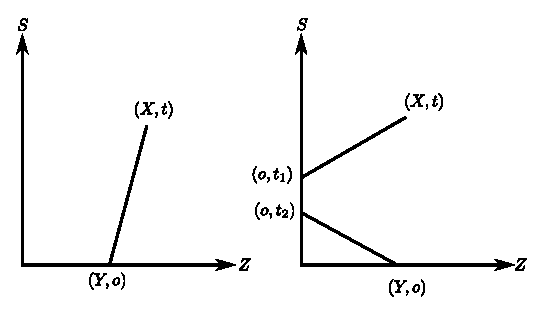
\includegraphics[scale=0.9]{figures/figure-art8.eps}
\end{figure}
 Let $u_{0}(x)\in L^{\infty}(0,\infty)$ and $\lambda(t)$ is continuous. Let $\lambda^{+}(t)$ be defined by
 \eqref{art8-eq-1.14} and let
 \begin{equation}\label{art8-eq-1.16}
 \alpha =\left\{
 \begin{aligned}
&\infty \quad\text{if}\quad f(u)\quad \text{satisfies}\quad (H_{1})\\
&1\quad  \text{if}\quad f(u)\quad \text{satisfies}\quad (H_{2})
 \end{aligned}
\right.
 \end{equation}
For each fixed $(x,y,t)$, $x \geq 0$, $y\geq 0$, define
\begin{equation}\label{art8-eq-1.17}
\bQ(\bx, \by, \bt) = \min\limits_{\beta \epsilon \calC_{\alpha}(x,y,t)}[-\int_{\{s:\beta(s)=0\}} f(\lambda^{+}(s))ds + \int_{\{s:\beta(s)>0\}}f^{\star}\left(\dfrac{\rm{ds}}{\partial{\rm s}}\right){\rm ds}]
\end{equation}
It can be shown that $Q(x,y,t)$ is Lipschitz continous function. Let
\begin{equation}\label{art8-eq-1.18}
Q_{1}(x,y,t)= \dfrac{\partial}{\partial x}Q(x,y,t)
\end{equation} 
and
\begin{equation}\label{art8-eq-1.19}
U(x, t) = \min\limits_{0 \leq < \infty}\left[\int_{0}^{y}u_{0}(z)dz + Q(x,y,t)\right].
\end{equation}
For each fixed $(x,t)$ there may be several minimisers for \eqref{art8-eq-1.19}. Define
\begin{equation}\label{art8-eq-1.20}
y_{0}^{-}(x, t) =\min\{y_{0}(x,t)\}, y_{0}^{+}(x,t)=\max\{y_{0}(x,t)\}
\end{equation}

It can be shown  that (see \cite{art8-key5}), for each fixed $t> 0$, $y_{0}^{-}(.,t)$ and $y_{0}^{+}(.,t)$ are left continuous and right continuous respectively, and both are continuous except on a comman denumerable set of points of $x$ and at the points of continuity
$$
y_{0}^{+}(x, t)= y_{0}^{-}(x,t)
$$ 
Define
\begin{equation}\label{art8-eq-1.21}
u(x,t)=Q_{1}(x, y_{0}(x,t),t)\; \text{and}
\end{equation}
\begin{equation}\label{art8-eq-1.22}
u(x \pm, t) =Q_{1}(x,y_{0}^{\pm}(x,t),t)
\end{equation}
Clearly $u(x,t)$ is well defined a.e $x>0$, $t>0$ and $u(x\pm, t)$ is well defined for all $x>0$, $t>0$. Our main result is the following theorem.

\begin{theorem}\label{art8-thm-2}
Let $u(x,t)$ be given by \eqref{art8-eq-1.21} and \eqref{art8-eq-1.22}, then it is the solution of \eqref{art8-eq-1.1}
\eqref{art8-eq-1.10}, \eqref{art8-eq-1.13} and \eqref{art8-eq-1.3}. 
\end{theorem}
 Here we remark that viscosity solution of Hamilton Jacobi equation with Neumann boundary condition (see Lions \cite{art8-key11, art8-key12}).
 \begin{equation}\label{art8-eq-1.23}
 \left\{
\begin{aligned}
&U_{t}+ f(U_{x})=0\\
&U(x, 0) =U_{0}(x)\\
&``U_{x}(0,t)= \lambda(t)"
\end{aligned}
\right.
 \end{equation}
is closely related to our problem. In fact the proof of theorem \ref{art8-thm-2} shows the following result.

\begin{theorem}\label{art8-thm-3}
The function $U(x, t)$ defined by
\begin{equation}\label{art8-eq-1.24}
U(x,t)= \min\limits_{0 \leq y \leq \infty}[U_{0}(y) + Q(x, y,t)]
\end{equation}
\end{theorem}
 is a viscosity solution of \eqref{art8-eq-1.23}.

Here $Q(x,y,t)$ is defined the same way a \eqref{art8-eq-1.17}.

We arrived at these results,by first working out two examples namely the Burgers equation \cite{art8-key3} and the Lax's equation \cite{art8-key4}.

\section{Burgers Equation}\label{art8-sec-2}
In this section, we conside the Burgers equation in $x > 0$, $t>0$
\begin{equation}\label{art8-eq-2.1}
\left\{
\begin{aligned}
&u_{t} + \left(\dfrac{u^{2}}{2}\right)_{x} = \dfrac{\epsilon}{2}u_{xx},\\
&u(x,0)=u_{0}(x),\\
&u(0,t) = \lambda(t),
\end{aligned}
\right.
\end{equation}
Let us define
\begin{equation}\label{art8-eq-2.2}
U^{\epsilon}(x,t) = -\int_{x}^{\infty} u(y,t)dy, U_{0}(y) = -\int_{0}^{\infty} u_{0}(y)dy.
\end{equation}
Then \eqref{art8-eq-2.1} becomes
\begin{equation}\label{art8-eq-2.3}
\left\{
\begin{aligned}
&U_{t}+\left(\dfrac{U_{x}^{2}}{2}\right) =\tfrac{\epsilon}{2}U_{xx},\\
&U(x, 0)=U_{0}(x),\\
&U_{x}(0,t)= \lambda(t).
\end{aligned}
\right.
\end{equation}
by the Hopf-Cole transformation
\begin{equation}\label{art8-eq-2.4}
V=e^{-\tfrac{1}{\epsilon}U,}
\end{equation}
We can linearize the problem \eqref{art8-eq-2.3}
\begin{equation}\label{art8-eq-2.5}
\left\{
\begin{aligned}
&V_{t} =\tfrac{\epsilon}{2}V_{xx},\\
&\epsilon V_{x}(0, t)+\lambda(t) V(0,t) = 0,\\
&V(x,0)= e^{-\frac{1}{\epsilon}U_{0}(x)}.
\end{aligned}
\right.
\end{equation}
When $\lambda(t)= \lambda$, a constant, the solution of \eqref{art8-eq-2.5} can be explicitly written down:
\begin{equation}\label{art8-eq-2.6}
\begin{split}
V^{\epsilon}(x,t) = \dfrac{1}{(2\pi t \epsilon )^{1/2}}\left[\int_{0}^{\infty} e^{\tfrac{-1}{\epsilon}\left[U_{0}(y)+ \dfrac{(x-y)^{2}}{2t}\right]}dy\right] +\\
+ \int_{0}^{\infty}e^{\tfrac{-1}{\epsilon}\left[U_{0}(y)+ \dfrac{(x-y)^{2}}{2t}\right]}dy +
\dfrac{2(\lambda/\epsilon)}{(2\pi t\epsilon)^{1/2}}\\ \int_{0}^{\infty} \int_{y}^{\infty} e^{-\dfrac{1}{\epsilon}\left[\lambda(y-z)+U_{0}(y) +\dfrac{(y+z)^{2}}{2t}\right]}dzdy.
\end{split}
\end{equation}
From \eqref{art8-eq-2.4}, we have
\begin{equation}\label{art8-eq-2.7}
U^{\epsilon}(x, t)= -\epsilon\log(V^{\epsilon}(x, t)).
\end{equation}
Substituting \eqref{art8-eq-2.6} in \eqref{art8-eq-2.7}, we have an explicit formula for $U^{\epsilon}(x,t)$. Using the method of stationary phase one can show that the $\lim_{\epsilon \rightarrow 0}U^{\epsilon}\break (x, t)=U(x,t)$ exists and is given by \eqref{art8-eq-1.24}. The general variable boundary data $\lambda{t}$ can be treated by using a comparison theorem and some elementary convex analysis. The details can be found in \cite{art8-key3}.

\section{Lax's equation}\label{art8-sec-3}

In this section, we consider the Lax's equation
\begin{equation}\label{art8-eq-3.1}
u_{t}+ \left(\log \left[ae^{u} + be^{-u}\right]_{x}\right)= 0,
\end{equation}
In $x>0$, $t>0$. In the case of no boundary Lax \cite{art8-key9} studied this example by a difference scheme. We consider the case with boundary. Let
\begin{equation}\label{art8-eq-3.2}
u_{k}^{n}\simeq u(k\Delta, n\Delta), k=0,1,2,\ldots,n = 0,1,2,\ldots
\end{equation}
$\Delta$ being the mesh size. Let $u^{\Delta}(x,t)$ be the approximate solution defined by
\begin{equation}\label{art8-eq-3.3}
\left\{
\begin{aligned}
&u_{k}^{n+1} = u_{k}^{n} + \left[g(u_{k-1}^{n}, u_{k}^{n})-g(u_{k}^{n}, u_{k+}^{n})\right]\\
&u_{k}^{0} = u_{0}(k(\Delta))\\
&u_{0}^{n} = \lambda(n\Delta)
\end{aligned}
\right.
\end{equation}
where the numerical flux $g(u,v)$ is given by
\begin{equation}\label{art8-eq-3.4}
g(u,v) = \log \left[ae^{u} + be^{-v}\right].
\end{equation}
Let
\begin{equation}\label{art8-eq-3.5}
U_{k}^{n} = -\sum\limits_{j=k}^{\infty} u_{j}^{n}, U_{k}^{k} = -\sum_{j=k}^{\infty} u_{0}(j \Delta), U_{k}^{n}= \log V_{k}^{n},
\end{equation}
then from \eqref{art8-eq-3.3}, we get
\begin{equation}\label{art8-eq-3.6}
\left\{
\begin{aligned}
&V_{k}^{n+1} =aV_{k+1}^{n} +bV_{k-1}^{n}, \quad n=1,2,\ldots,k=1,2,3,\ldots\\
&V_{k}^{0}=e^{-U_{k}^{0}}, \qquad \qquad  k=0,1,2,\\
&V_{0}^{n} =e^{\lambda(n)}V_{1}^{n}, \qquad  \quad n=1,2,\ldots  
\end{aligned}
\right.
\end{equation}
when $\lambda = \lambda(t)$, a constant, an explicit formula can be obtained for the solution of \eqref{art8-eq-3.6} namely

\begin{equation}\label{art8-eq-3.7}
V_{k}^{n}=\left\{
\begin{aligned}
&e^{(n-k)\lambda}\sum\limits_{q=0}^{n}\binom{n}{q}a^{q}b^{n-q}V_{2n-2q}^{0}\\
&\qquad + \sum\limits_{j=0}^{n-k-1} e^{j\lambda}S_{n,k+j},\quad \text{if} \; n > k\\
&\sum\limits_{q=0}^{n}\binom{n}{q}a^{q}b^{n-q}V_{n+k-2q}^{0},\quad \text{if} \; n\leq k
\end{aligned}
\right.
\end{equation}
where
\begin{align*}
S_{n,k} &=\sum\limits_{q=0}^{r}C_{q,k}^{n}a^{q}b^{n-q}\left(V_{n+k-2q}^{0}-e^{\lambda}V_{n+k+1-2q}^{0}\right)\\
r &= 
\begin{cases}
 \dfrac{n+k+-1}{2}\quad \text{if}\quad (n+k)\quad \text{is odd}\\
 \dfrac{n+k+-2}{2}\quad \text{if}\quad (n+k)\quad \text{is even}\\
\end{cases}\\
C_{q,k}^{n}&=
\begin{cases}
\binom{n}{q} \quad , \text{if}\; \quad q \leq k-1\\
\binom{n}{q}-\binom{n}{q-k},\; \text{if}\; q \geq k
\end{cases}
\end{align*}
and
$$
\binom{n}{j} = \dfrac{n!}{j!(n-j)!}
$$
By retracing the transformation \eqref{art8-eq-3.5}, and using \eqref{art8-eq-3.7}, we get an explicit formula for $U^{\Delta}(x,t)= -\int_{x}^{\infty}u^{\Delta}(y,t)dy$. Using Stirling's asymptotic formula one can study the limit, $\lim_{\Delta \rightarrow 0}U^{\Delta}(x,t) =U(x, t)$ and show that $U(x,t)$ is given by \eqref{art8-eq-1.24}. As in the case the Burgers Equation here agin once can prove a comparison theorem and with the help of this comparison theorem general variable $\lambda(t)$ can be treated. The details are omitted and can be found in \cite{art8-key8}.

\section{Proof of Main theorem}\label{art8-sec-4}
The examples of last two section suggest the formula for the case of general convex $f(u)$.

Following Lax \cite{art8-key9}, we introduce
\begin{equation}\label{art8-eq-4.1}
u_{N}(x, t) = \dfrac{\int_{0}^{\infty}Q_{1}(x,y,t)e^{-N[u_{0}(y)+Q(x,y,t)]}dy}{\int_{0}^{\infty}e^{-N[U_{0}(y)+Q(x,y,t)]}dy}
\end{equation}
\begin{equation}\label{art8-eq-4.2}
f_{N}(x,t) =  \dfrac{\int_{0}^{\infty} f(Q_{1}(x,y,t))e^{-N[U_{0}(y)+Q(x,y,t)]}dy} {\int_{0}^{\infty} e^{-N[U_{0}(y) +q(x,y,t)]}dy}
\end{equation}
\begin{equation}\label{art8-eq-4.3}
V_{N}(x,t) = \int_{0}^{\infty}e^{-N[U_{0}(y) + Q(x,y,t)]dy}.
\end{equation}
\begin{equation}\label{art8-eq-4.4}
U_{N}(x,t) = -\dfrac{1}{N}\log V_{N}.
\end{equation}
where $U_{0}(x)$, $Q(x,y,t)$,$Q_{1}(x,y,t)$ are defined in Sec \ref{art8-sec-1}. It is clear that
\begin{align}\label{art8-eq-4.5}
\begin{cases}
\lim_{N\rightarrow \infty}u_{N}(x,t)&= Q_{1}(x,y_{0}(x,t),t) \quad \text{a.e} (x,t)\\
\lim_{N\rightarrow \infty}f_{N}(x,t)&= f[Q_{1}(x,y_{0}(x,t),t)]\quad \text{a.e} (x,t)
\end{cases}
\end{align}
where $y_{0}(x,t)$ minimises \eqref{art8-eq-1.19} and
\begin{equation}\label{art8-eq-4.6}
\lim\limits_{N \rightarrow \infty}U_{N}(x,t)=U(x,t),
\end{equation}
and
\begin{equation}\label{art8-eq-4.7}
\dfrac{\partial U}{\partial x} = Q_{1}(x, y_{0}(x,t),t).
\end{equation}
It can be shown that
\begin{equation}\label{art8-eq-4.8}
\int_{0}^{\infty} \int_{0}^{\infty} (u_{N}\phi_{t} + f_{N})dx dt =0
\end{equation}
for all test function $\phi \in C_{0}^{\infty}(0,\infty) \times (0, \infty)$.

Let $N\rightarrow \infty$ and use \eqref{art8-eq-4.5} we get from \eqref{art8-eq-4.8}
\begin{equation}\label{art8-eq-4.9}
u(x,t) =Q_{1}(x, y_{0}(x,t),t)
\end{equation}
solves \eqref{art8-eq-1.1} in distribution. It can be shown that $u(x,t)$ defined by \eqref{art8-eq-4.9} satisfies initial condition \eqref{art8-eq-1.10} boundary condition \eqref{art8-eq-1.13} and entropy condition \eqref{art8-eq-1.3}. The details can be found in \cite{art8-key5}.

\begin{thebibliography}{99}
\bibitem{art8-key1} Bardos, C. Leroux, A.Y. and Nedelec, J.C., \textit{First order quasilinear equations with boundary conditions}, Comm. Partial Differential equations {\bf 4} (1979) 1017-1034.

\bibitem{art8-key2} Hopf, E. \textit{The partial differential equation}$ u_{t}uu_{x}=\mu U_{xx}$, Comm. Pure and Appl. Math {\bf 13} (1950) 201-230.
\bibitem{art8-key3} Joseph, K.T. \textit{Burgers equation in the quarter plane, a formula for the weak limit}, Comm. Pure and Appl. Math {\bf 41} (1988) 133-149.
\bibitem{art8-key4} Joseph, K. T. and Veerappa Gowda, G. D., \textit{Explicit-formula for the limit of a difference approximation}, Duke Math. J. {\bf 61} (1990) 369-393.

\bibitem{art8-key5} Joseph, K. T. and Veerappa Gowda, G. D., \textit{Explicit-formula for the solution of convex conservation laws wit boundary condition}, Duke Math. J. {\bf 62} (1991) 401-416.

\bibitem{art8-key6} Joseph, K. T. and Veerappa Gowda, G.D., \textit{Solution of convex conservation laws is a strip}, Proc Ind. Acad. Sci, {\bf 102}, 1,(1992) 29-47.

\bibitem{art8-key7} Kruskov, S. \textit{First order quasilinear equations with several space variables}, Math. USSR Sb,
 {\bf 10} (1970) 217-273.
\bibitem{art8-key8} Lax, P.D., \textit{Weak solutions of non linear hyperbolic equations and their numerical computation}, Comm. Pure Appl. Math {\bf 7} (1954) 159-193.

\bibitem{art8-key9} Lax, P. D: \textit{Hyperbolic Systems of Conservation laws II}, Comm. Pure Appl. Math. {\bf 10} (1957) 537-566.
 
\bibitem{art8-key10} Lefloch, P.,\textit{Explicit-formula for Scalar non-linear Conservation laws with boundary condition}, Math Methods in Appl. Sci {\bf 10} (1988) 265-287.

\bibitem{art8-key11} Lions, P.L., \textit{Generalized solutions of Hamilton-Jacobi equation}, Pitman Lecture Notes, Pitman, London (1982).

\bibitem{art8-key12} Lions, P.L., \textit{Neumann type boundary conditions for Hamilton-Jacobi equations}, Duke Math. J.
{\bf 52} (1985) 793-820.

\bibitem{art8-key13} Quinn, B., \textit{Solutions with shocks: an example of $L^{1}$- contraction semi-group}, Comm. Pure Appl. Math. {\bf 24} (1971) 125-132.

\bibitem{art8-key14} Oleinik, O.,\textit{Discontinuous solutions of non-linear differential equation}, Usp. Mat. Nauk, (N.S), {\bf 12} (1957) 3-73; English transl. in AMS Transl. Ser. 2, {\bf 26} (1957) 95-172.
\end{thebibliography}

\begin{flushleft}
TIFR Centre

P.B. No.1234

IISc. Campus

Bangalore 560 012
\end{flushleft}
